\section{Italian Grand Prix}

\subsection{Circuit Analysis}

\textbf{Circuit Name:} Autodromo Nazionale di Monza (Monza, Italy) \\
\textbf{Length:} 5.793 km - \textbf{Laps:} 53 - \textbf{Total Distance:} 306.720 km

\begin{figure}[H]
    \centering
    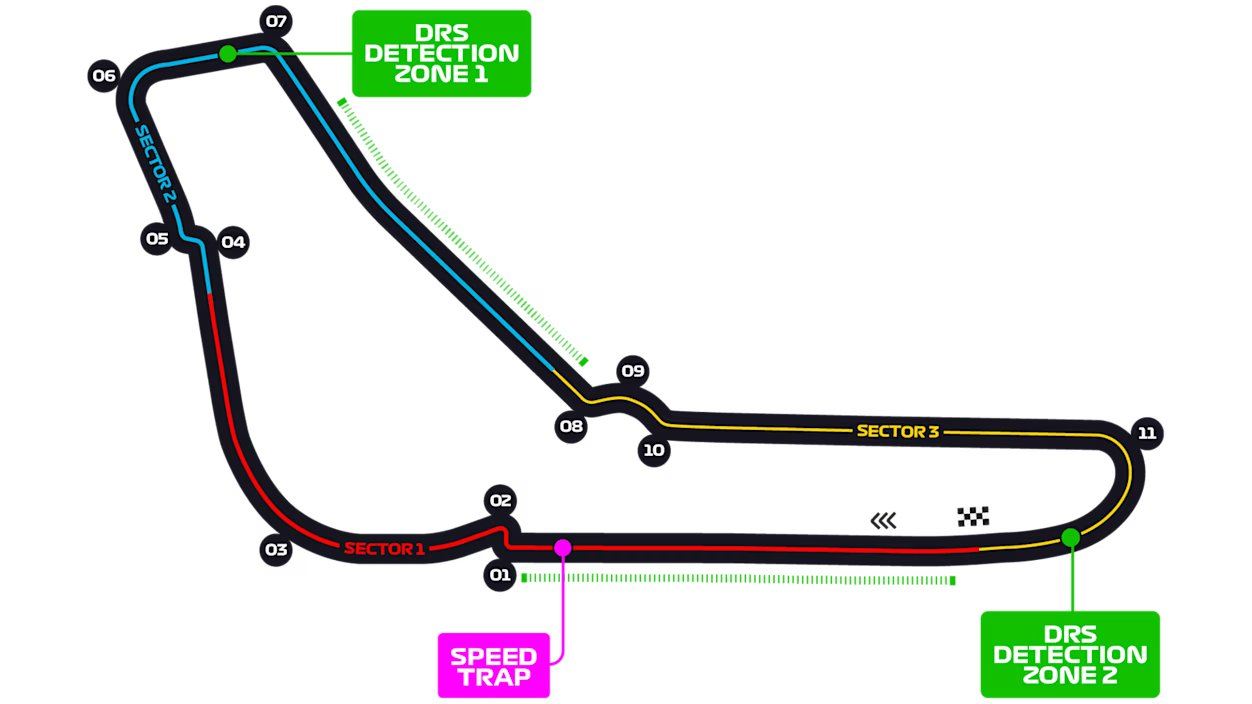
\includegraphics[width=0.75\linewidth]{images/16.Italy_Circuit.jpg}
\end{figure}

\begin{itemize}
    \item \textbf{Lap Record} : 1:18.887 (2020, Lewis Hamilton – Mercedes).
    
    \item \textbf{Number of Corners \& Key Features} : 11 turns (7 right, 4 left). \\
    Known as the “Temple of Speed”: long straights, chicanes (Rettifilo, Roggia), fast Lesmo corners, Ascari chicane, and the iconic Parabolica. \\
    Cars run minimum downforce to maximise top speed.
    
    \item \textbf{Braking Zones \& Traction} : Heavy braking zones at Turn 1 (Rettifilo) and Turn 4 (Roggia). \\
    Traction crucial out of Parabolica to carry speed onto main straight.
    
    \item \textbf{DRS \& Overtaking} : Two DRS zones (main straight, between Lesmo 2 and Ascari). \\
    Main overtaking into Rettifilo chicane, Ascari also provides opportunities.
    
    \item \textbf{Tyre Degradation \& Strategy} : Low tyre wear overall, but traction zones stress rears. \\
    One-stop possible but risky, two-stop often preferred.
    
    \item \textbf{Weather \& Environment} : Warm, stable late-summer weather. \\
    Huge tifosi support makes Monza Ferrari’s home fortress.
\end{itemize}

\textbf{Strategic Summary :} Monza rewards straight-line efficiency, braking stability, and clean pit execution. Track position is critical given DRS trains and limited overtaking beyond Turn 1.


\subsection{Race Analysis}

\textbf{Date:} 1 September 2024 — 15:00 local time 

\begin{itemize}
    \item \textbf{Qualifying Summary} : \textbf{Pole Position:} Lando Norris (McLaren) – 1:19.327. \\
    Grid: Piastri 2nd, Russell 3rd, Leclerc 4th.\\
    Franco Colapinto debuted with Williams, replacing Sargeant.
    
    \item \textbf{Race Summary} : \textbf{Winner: Charles Leclerc (Ferrari)}. \\
    \textbf{Podium:} 1. Leclerc - 2. Piastri - 3. Norris. \\
    Verstappen salvaged P6 in a difficult weekend for Red Bull.
    
    \item \textbf{Strategies} : 
    - Ferrari: Leclerc bold one-stop (Medium–Hard, 38 laps on hards). Perfect tyre management secured win. \\
    - McLaren: Piastri led early, forced to pit twice, Norris attempted undercut on Leclerc but lost track position. Both lacked tyre longevity. \\
    - Mercedes: Hamilton and Russell solid but lacked pace to fight podium. \\
    - Red Bull: Verstappen struggled on degradation, Pérez P8. \\
    - Midfield: Albon P9 strong for Williams. Haas in points despite penalties.
    
    \item \textbf{Performance Trends} :  
    \textbf{Ferrari:} Brilliant strategy and execution, Leclerc calm under pressure. Sainz strong support in P4. \\
    \textbf{McLaren:} Fastest in raw pace but outsmarted strategically. \\
    \textbf{Mercedes:} Consistent, but podium pace lacking. \\
    \textbf{Red Bull:} Fourth-best team — Verstappen frustrated, Pérez mediocre. \\
    \textbf{Midfield:} Williams (Albon) reliable, Haas scrappy points, Aston Martin invisible.
    
    \item \textbf{Championship Impact} : \textbf{Drivers:} Verstappen 303 pts, Norris 241, Leclerc 217. \\
    \textbf{Constructors:} Red Bull 446, McLaren 438, Ferrari 407, Mercedes 292
\end{itemize}

\textbf{Key Takeaway :} Charles Leclerc delivered an emotional victory at Monza with a masterful one-stop strategy, delighting the tifosi. McLaren proved the fastest team but paid for higher tyre wear. Red Bull faltered again, leaving Verstappen under pressure as the title fight tightened dramatically.

\subsection{Link \& Takeaway}

\begin{itemize}
    \item Ferrari’s home win emphasized strategic brilliance and Leclerc’s calm under pressure. 
    \item McLaren lost a win despite dominance in qualifying — tyre management still a weakness. 
    \item Red Bull continued to struggle, raising concerns about their position as championship leaders. 
    \item Mercedes remained consistent but lacked podium pace.
    \item The championship battle tightened further: Verstappen still leads but Norris, Leclerc, and Piastri are closing in.
\end{itemize}
